

This model was designed following the \textit{General Responsibility Assignment Software Patterns} (GRASP). The GRASP design principles provide guidelines for object-oriented software design and are well suited for a project such as this. The main focus of the principles, like the name states, is assigning responsibilities to the appropriate objects in the model. The basic roles in GRASP can be divided into \textit{knowing} and \textit{doing}. The design of the loon model is simple so the division was straight forward:
\begin{itemize}
\item[BALLOON:]
    \subitem Knows: A balloon object knows its own location, altitude and in which wind layer it is currently located.
    \subitem Does: A balloon object can move with the wind. It gets the wind vectors from the wind layer in which it is located. 

\item[WIND LAYER:]

    \subitem Knows: A wind layer object knows its own identification number, as well as the wind vector at any given place in the grid.
    \subitem Does: A wind layer does nothing but provide access to its data.

\item[WORLD:]

    \subitem Knows: The world know about the status of the simulation and how many steps have been taken. It collects statistical data about the grid in which the balloons hover. 
    \subitem Does: The world has access to all balloons and wind layers and is the controller of the simulation. The world initiates all decisions and movements of every balloon. 

\end{itemize}

The Balloon and WindLayer are expert classes while World is a controller class in this model. The algorithms developed during this project will be centralized, i.e controlled by an entity with knowledge of the entire system and access to all objects. This limits the balloons' responsibility to simply stay in the air, take commands and supply Internet coverage.

\begin{figure}[H]
    \centering
    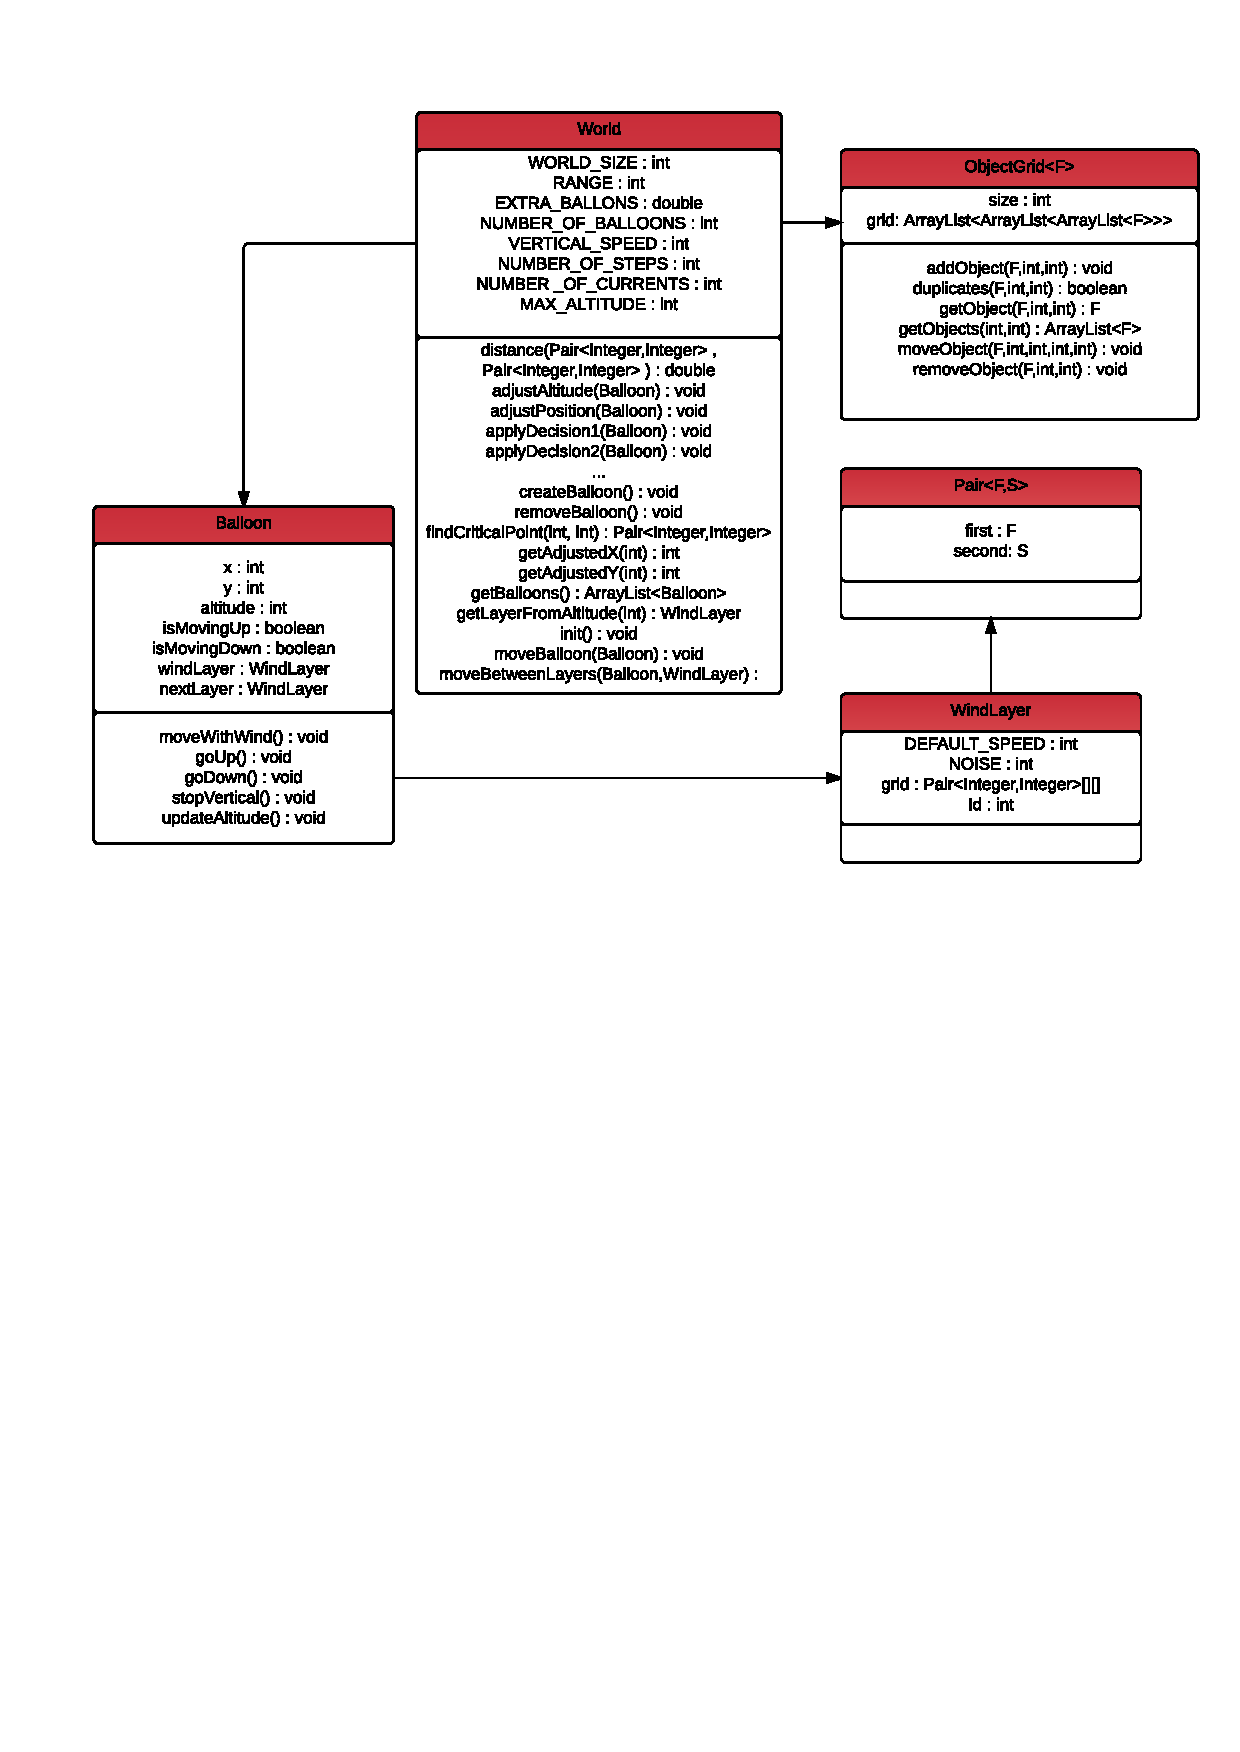
\includegraphics[width=\textwidth, trim= 1cm 14cm 0cm 0cm, clip]{graphics/classDiagram.pdf}
    \caption{Class Diagram}
    \label{fig:class_diagram}
\end{figure}


\begin{figure}[H]
    \centering
    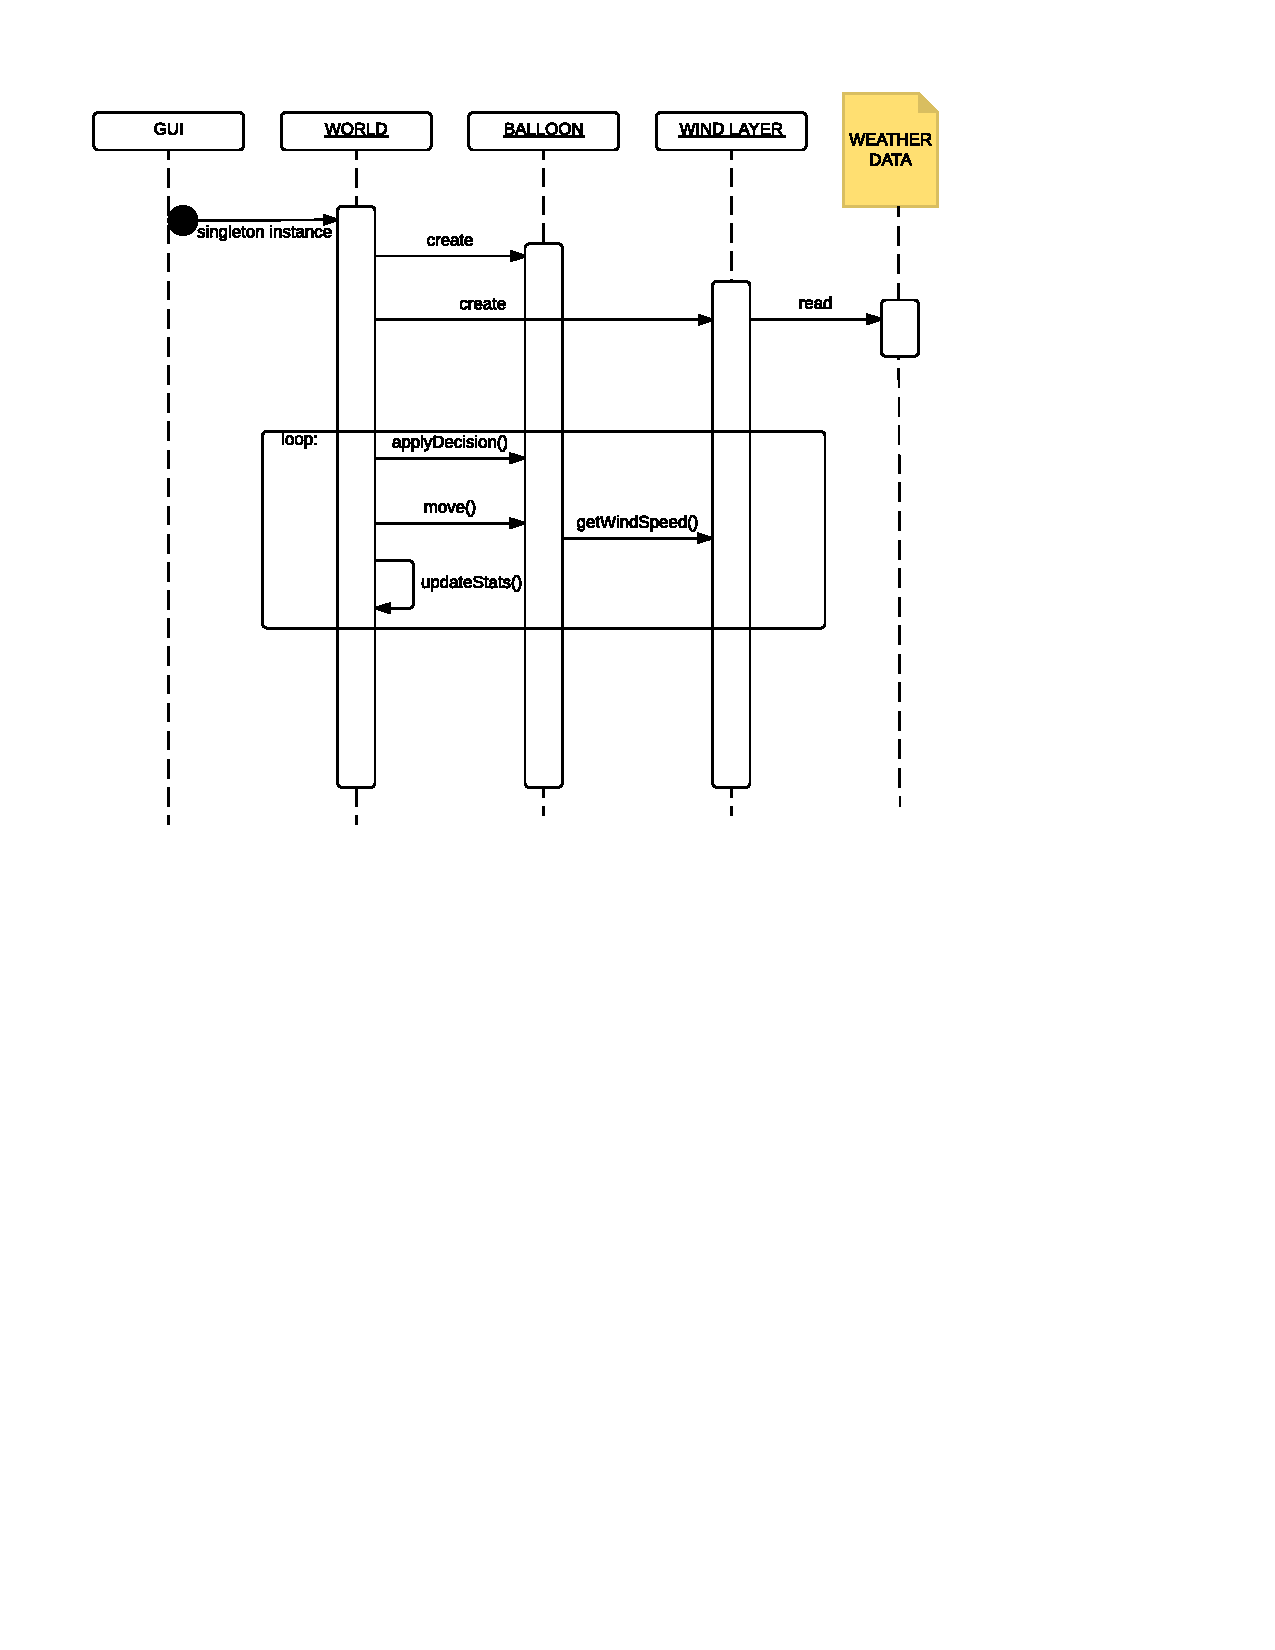
\includegraphics[width=\textwidth, trim= 1cm 12cm 4cm 1cm, clip]{graphics/sequenceDiagram.pdf}
    \caption{Simplified Sequence Diagram}
    \label{fig:seq_diagram}
\end{figure}

